\documentclass[dvipsnames,hidelinks]{beamer}

  % Enables the use of colour.
  \usepackage{xcolor}
  % Syntax high-lighting for code. Requires Python's pygments.
  \usepackage{minted}
  % Enables the use of umlauts and other accents.
  \usepackage[utf8]{inputenc}
  % Diagrams.
  \usepackage{tikz}
  % Settings for captions, such as sideways captions.
  \usepackage{caption}
  % Symbols for units, like degrees and ohms.
  \usepackage{gensymb}
  % Latin modern fonts - better looking than the defaults.
  \usepackage{lmodern}
  % Allows for columns spanning multiple rows in tables.
  \usepackage{multirow}
  % Better looking tables, including nicer borders.
  \usepackage{booktabs}
  % More math symbols.
  \usepackage{amssymb}
  % More math fonts, like mathbb.
  \usepackage{amsfonts}
  % More math layouts, equation arrays, etc.
  \usepackage{amsmath}
  % More theorem environments.
  \usepackage{amsthm}
  % More column formats for tables.
  \usepackage{array}
  % Adjust the sizes of box environments.
  \usepackage{adjustbox}
  % Better looking single quotes in verbatim and minted environments.
  \usepackage{upquote}
  % Better blank space decisions.
  \usepackage{xspace}
  % Better looking tikz trees.
  \usepackage{forest}
  % URLs.
  \usepackage{hyperref}
  % For plotting.
  \usepackage{pgfplots}
  % For more font sizes.
  \usepackage{anyfontsize}
  
  % Various tikz libraries.
  % For drawing mind maps.
  \usetikzlibrary{mindmap}
  % For adding shadows.
  \usetikzlibrary{shadows}
  % Extra arrows tips.
  \usetikzlibrary{arrows.meta}
  % Old arrows.
  \usetikzlibrary{arrows}
  % Automata.
  \usetikzlibrary{automata}
  % For more positioning options.
  \usetikzlibrary{positioning}
  % Creating chains of nodes on a line.
  \usetikzlibrary{chains}
  % Fitting node to contain set of coordinates.
  \usetikzlibrary{fit}
  % Extra shapes for drawing.
  \usetikzlibrary{shapes}
  % For markings on paths.
  \usetikzlibrary{decorations.markings}
  % For advanced calculations.
  \usetikzlibrary{calc}
  % For decorations on paths.
  \usetikzlibrary{decorations.text}
  
  % GMIT colours.
  \definecolor{gmitblue}{RGB}{20,134,225}
  \definecolor{gmitred}{RGB}{220,20,60} 
  \definecolor{gmitgrey}{RGB}{67,67,67}
  
  % Change some style options.
  \usetheme{metropolis}
  % Tell minted to use the following colour scheme. 
  \usemintedstyle{manni}

  \metroset{sectionpage=simple, numbering=none, block=fill}

  % Change the default theme colours.
  \setbeamercolor{normal text}{fg=darkgray, bg=white}
  \setbeamercolor{alerted text}{fg=gmitred, bg=white}
  \setbeamercolor{example text}{fg=gmitblue, bg=white}
  \setbeamercolor{frametitle}{fg=white, bg=gmitblue}
  \setbeamercolor*{item}{fg=gmitblue}
  % Use a better math mode font.
  \usefonttheme[onlymath]{serif}

  % \citeurl can be used to a clickable short url to a slide as a reference.
  \renewcommand\footnoterule{}
  \newcommand{\citeurl}[1]{\let\thefootnote\relax\footnotetext{\tiny \textcolor{gmitgrey}{\href{http://#1}{#1}}}}
  \newcommand{\citeeg}[1]{\let\thefootnote\relax\footnotetext{\tiny \textcolor{gmitgrey}{#1}}}
  
  % Prevent minted from showing errors.
  \makeatletter
  \expandafter\def\csname PYGdefault@tok@err\endcsname{\def\PYGdefault@bc##1{{\strut ##1}}}
  \makeatother
  
  \setbeamertemplate{section page}
  {
      \begin{centering}
      \begin{beamercolorbox}[sep=12pt,center]{part title}
      \usebeamerfont{section title}\insertsection\par
      \end{beamercolorbox}
      \end{centering}

      \begin{center}
        \small ian.mcloughlin@gmit.ie
      \end{center}
  } 


\begin{document}
  \section{Learning}

\begin{frame}{Memorize these symbols}
  \vspace{8mm}
  \centering
  \begin{adjustbox}{width=0.8\columnwidth, keepaspectratio}
    \begin{tikzpicture}
      \draw[thick,                color=gmitblue] (0,0) -- (1,0) -- (1,1);
      \draw[thick,shift={(0,-2)} ,color=gmitblue] (0,1) -- (0,0) -- (1,0) -- (1,1);
      \draw[thick,shift={(0,-4)} ,color=gmitblue] (0,1) -- (0,0) -- (1,0);
      \draw[thick,shift={(0,-6)} ,color=gmitblue] (0,1) -- (1,1) -- (1,0) -- (0,0);
      \draw[thick,shift={(4, 0)} ,color=gmitblue] (0,0) -- (0,1) -- (1,1) -- (1,0) -- (0,0);
      \draw[thick,shift={(4,-2)} ,color=gmitblue] (1,1) -- (0,1) -- (0,0) -- (1,0);
      \draw[thick,shift={(4,-4)} ,color=gmitblue] (0,1) -- (1,1) -- (1,0);
      \draw[thick,shift={(4,-6)} ,color=gmitblue] (0,0) -- (0,1) -- (1,1) -- (1,0);
      \draw[thick,shift={(8, 0)} ,color=gmitblue] (0,0) -- (0,1) -- (1,1);
      \node at (-0.5, 0.5) {\Large $1.$};
      \node at (-0.5,-1.5) {\Large $2.$};
      \node at (-0.5,-3.5) {\Large $3.$};
      \node at (-0.5,-5.5) {\Large $4.$};
      \node at ( 3.5, 0.5) {\Large $5.$};
      \node at ( 3.5,-1.5) {\Large $6.$};
      \node at ( 3.5,-3.5) {\Large $7.$};
      \node at ( 3.5,-5.5) {\Large $8.$};
      \node at ( 7.5, 0.5) {\Large $9.$};
    \end{tikzpicture}
  \end{adjustbox}
\end{frame}

\begin{frame}[standout]
  \begin{quote}
    Write down the symbols corresponding to the number 314,159.
  \end{quote}
\end{frame}

\begin{frame}
  \vspace{8mm}
  \centering
  %\begin{adjustbox}{width=0.8\columnwidth, keepaspectratio}
    \begin{tikzpicture}
      \draw[thick, color=gmitblue] (-2, 0) -- (4,0);
      \draw[thick, color=gmitblue] (-2, 2) -- (4,2);
      \draw[thick, color=gmitblue] ( 0,-2) -- (0,4);
      \draw[thick, color=gmitblue] ( 2,-2) -- (2,4);
      \node at (-1, 3) {\Large $1$};
      \node at ( 1, 3) {\Large $2$};
      \node at ( 3, 3) {\Large $3$};
      \node at (-1, 1) {\Large $4$};
      \node at ( 1, 1) {\Large $5$};
      \node at ( 3, 1) {\Large $6$};
      \node at (-1,-1) {\Large $7$};
      \node at ( 1,-1) {\Large $8$};
      \node at ( 3,-1) {\Large $9$};
    \end{tikzpicture}
  %\end{adjustbox}
\end{frame}

\begin{frame}[standout]
  \begin{quote}
    Knowledge is constructed as a result of the learner's activity. \\[8mm]
  \end{quote}

  {\scriptsize -- Teaching Teaching \& Understanding Understanding by Claus Brabrand}

\end{frame}

\begin{frame}{Zone of proximal development}
  \vspace{4mm}
  \centering
  \begin{adjustbox}{width=0.7\columnwidth, keepaspectratio}
    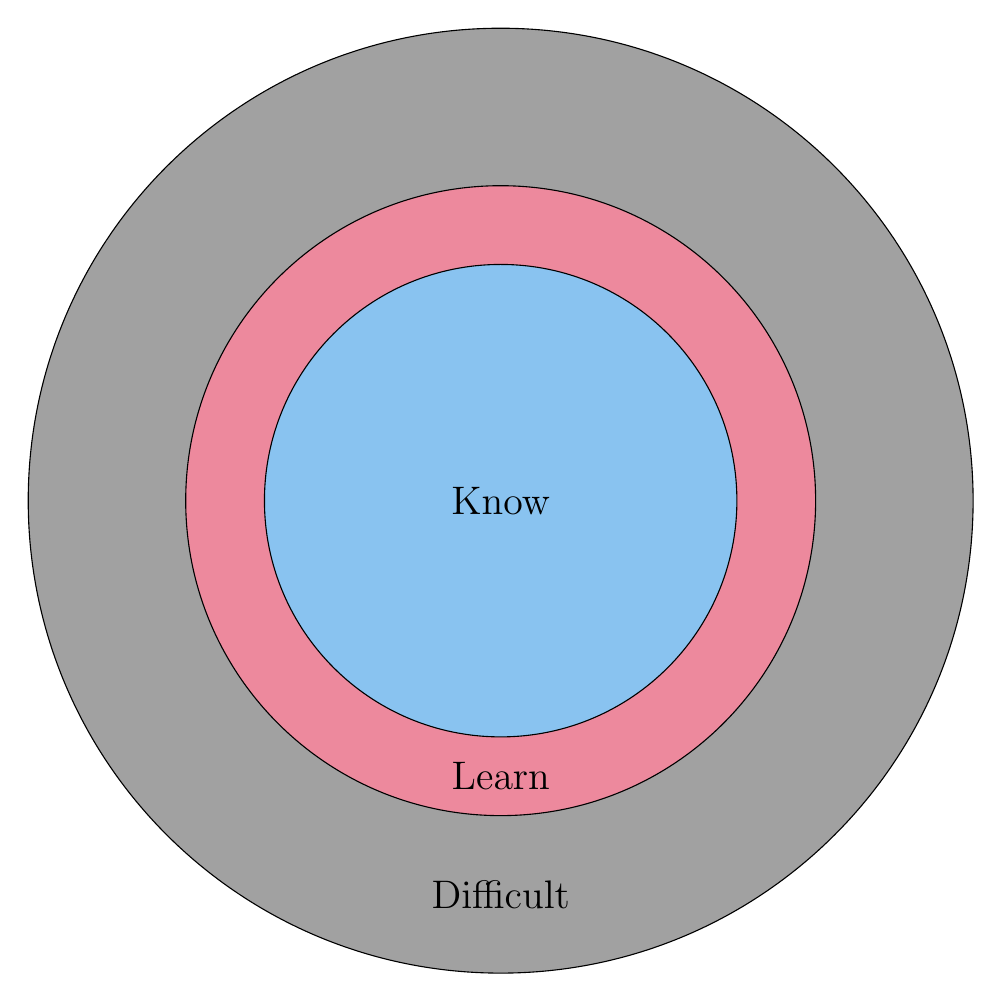
\begin{tikzpicture}
      \draw[fill=gmitgrey!50] (0,0) circle (6);
      \draw[fill=gmitred!50] (0,0) circle (4);
      \draw[fill=gmitblue!50] (0,0) circle (3);
      \node at (0,0) {\Large Know};
      \node at (0,-3.5) {\Large Learn};
      \node at (0,-5) {\Large Difficult};
    \end{tikzpicture}
  \end{adjustbox}
  
\end{frame} 
\end{document}